%------------------------------------------------------------------------------%

\usepackage{apresentacao}
\usepackage{mathconfig}
\usepackage{tabto}

\setlength{\parskip}{0.5\baselineskip}

\newcounter{exemplo}
\setcounter{exemplo}{0}

\makeatletter
\graphicspath  {{./figs/}}
\def\input@path{{./figs/}}
\makeatother

\newcommand{\D}[2]{\frac{\partial {#1}}{\partial {#2}}}
\newcommand{\DS}[2]{\frac{\partial^2 {#1}}{\partial {#2}^2}}
\newcommand{\DM}[3]{\frac{\partial^2 {#1}}{\partial {#2} \partial {#3}}}

%------------------------------------------------------------------------------%
\title {Curvas Paramétricas}
\author{\large Luis Alberto D'Afonseca}
\date  {Cálculo de Funções de Várias Variáveis I}

%------------------------------------------------------------------------------%
\begin{document}

%------------------------------------------------------------------------------%
\begin{frame}
    \titlepage
\end{frame}

%------------------------------------------------------------------------------%
\section{Introdução}

\framedgraphic{Trajetória}{trajeto_maps}{}

%------------------------------------------------------------------------------%
\begin{frame}{Gráfico de uma Função Real}
  Conjunto de pontos $(x, y) \in \R^2$ tais que \(y = f(x)\)

  \pause
  \vspace{\baselineskip}
  Para cada $x$, no domínio, existe \emph{um único} $y$ no contradomínio
\end{frame}

%------------------------------------------------------------------------------%
\begin{frame}{Gráfico de uma Função Real}
  \centering
  

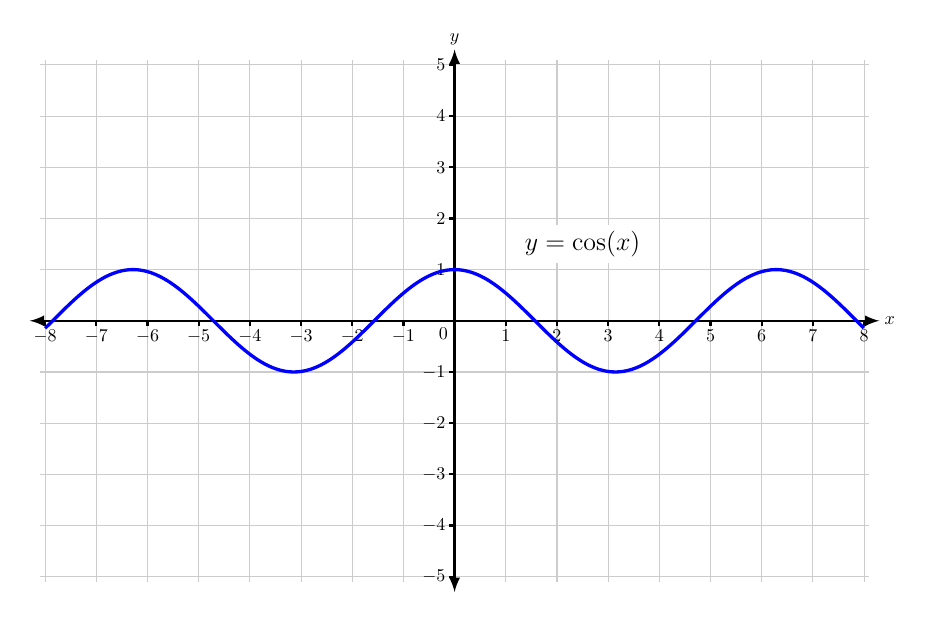
\begin{tikzpicture}[thick,scale=0.65, every node/.style={scale=0.65}]
  \def \minx {-8}
  \def \maxx {8}
  \def \miny {-5}
  \def \maxy {5}

  \draw[thin,black!20] (\minx-0.1,\miny-0.1) grid (\maxx+0.1,\maxy+0.1);

  \draw[thick, latex-latex] (\minx-0.3,0)--(\maxx+0.3,0);
  \draw[thick, latex-latex] (0,\miny-0.3)--(0,\maxy+0.3);
  \node at (\maxx+0.5,0) {$x$};
  \node at (0,\maxy+0.5) {$y$};

  \foreach \x in {\minx,...,-1}{
    \draw (\x,0)--(\x,-0.1);
    \node[below,black] at (\x,-0.05) {$\x$};
  }
  \foreach \x in {1,...,\maxx}{
    \draw (\x,0)--(\x,-0.1);
    \node[below,black] at (\x,-0.05) {$\x$};
  }
  \foreach \y in {\miny,...,-1}{
    \draw (0,\y)--(-0.1,\y);
    \node[left,black] at (-0.05,\y) {$\y$};
  }
  \foreach \y in {1,...,\maxy}{
    \draw (0,\y)--(-0.1,\y);
    \node[left,black] at (-0.05,\y) {$\y$};
  }
  \node[below left,black] at (0,0) {$0$};

  \draw[very thick, domain=\minx:\maxx, variable=\x, smooth, samples=300, blue]  plot ({\x},{cos(\x r)});

  \node at (2.5,1.5) [fill=white] {\Large $y=\cos(x)$};
\end{tikzpicture}

\end{frame}

%------------------------------------------------------------------------------%
\begin{frame}{Soluções de uma Equação}

  Uma expressão da forma
  \[
    G(x, y) = 0
  \]

  \pause
  \vspace{\baselineskip}
  Queremos \emph{todos os pares} $(x, y)$ que satisfazem a equação

  \pause
  \vspace{\baselineskip}
  Se faltar um, a solução está incompleta e portanto errada
\end{frame}

%------------------------------------------------------------------------------%
\begin{frame}{Soluções de uma Equação}
  \centering
  \input{grafico_equacao}
\end{frame}

%------------------------------------------------------------------------------%
\begin{frame}{Curvas Paramétricas}
  Funções de $\R$ em $\R^n$
  \[
  \left(\begin{array}{>{\,}c<{\,}}
    x \\[1mm]
    y
  \end{array}\right)
  =
  \left(\begin{array}{>{\,}c<{\,}}
    f(t) \\[1mm]
    g(t)
  \end{array}\right)
  \]

  \pause
  \vspace{\baselineskip}
  Podemos pensar na variável como o tempo e a curva como uma trajetória
\end{frame}

%------------------------------------------------------------------------------%
\begin{frame}{Curvas Paramétricas}
  \centering
  

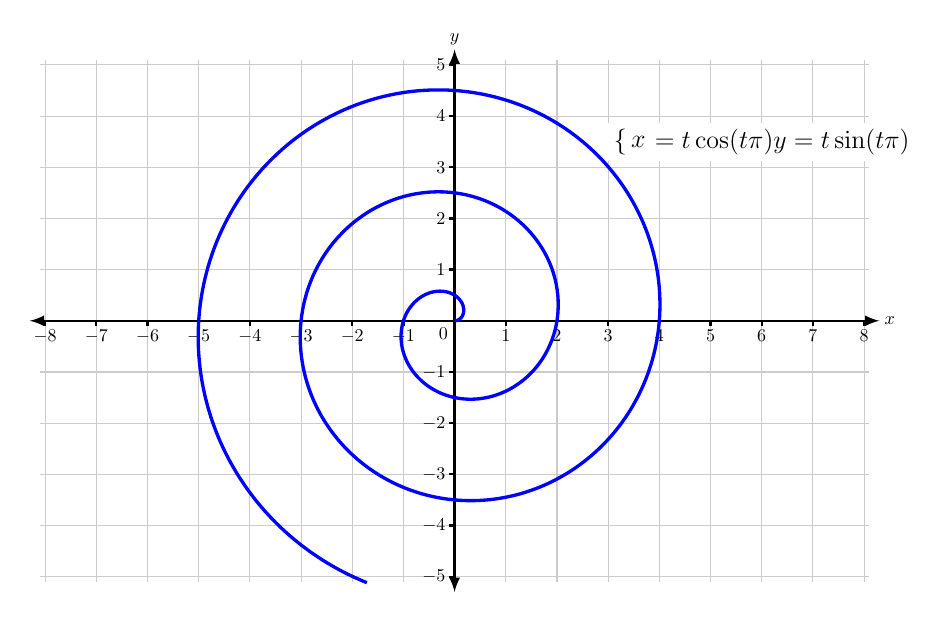
\begin{tikzpicture}[thick,scale=0.65, every node/.style={scale=0.65}]
  \def \minx {-8}
  \def \maxx {8}
  \def \miny {-5}
  \def \maxy {5}

  \draw[thin,black!20] (\minx-0.1,\miny-0.1) grid (\maxx+0.1,\maxy+0.1);

  \draw[thick, latex-latex] (\minx-0.3,0)--(\maxx+0.3,0);
  \draw[thick, latex-latex] (0,\miny-0.3)--(0,\maxy+0.3);
  \node at (\maxx+0.5,0) {$x$};
  \node at (0,\maxy+0.5) {$y$};

  \foreach \x in {\minx,...,-1}{
    \draw (\x,0)--(\x,-0.1);
    \node[below,black] at (\x,-0.05) {$\x$};
  }
  \foreach \x in {1,...,\maxx}{
    \draw (\x,0)--(\x,-0.1);
    \node[below,black] at (\x,-0.05) {$\x$};
  }
  \foreach \y in {\miny,...,-1}{
    \draw (0,\y)--(-0.1,\y);
    \node[left,black] at (-0.05,\y) {$\y$};
  }
  \foreach \y in {1,...,\maxy}{
    \draw (0,\y)--(-0.1,\y);
    \node[left,black] at (-0.05,\y) {$\y$};
  }
  \node[below left,black] at (0,0) {$0$};

  \draw[
    very thick,
    domain=0:5.4,
    variable=\t,
    smooth,
    samples=300,
    blue]
    plot ({\t*cos(\t*3.1415 r)},{\t*sin(\t*3.1415 r)});

  \node at (6,3.5) [fill=white]
  {
      \Large
      $
      \begin{cases}
        x = t \cos(t\pi) \\
        y = t \sin(t\pi)
      \end{cases}
      $
  };
\end{tikzpicture}

\end{frame}

%------------------------------------------------------------------------------%
\section{Curvas Paramétricas}

%------------------------------------------------------------------------------%
\begin{frame}{Definição em 2D}
  Se $x$ e $y$ são dados como funções
  \[
    x = f(t)
    \qquad
    y = g(t)
  \]
  sobre um intervalo $I$ de valores de $t$,
  \pause
  então o conjunto de pontos
  \[
    (x, y) = \big( f(t), g(t)\big)
  \]
  forma uma \emph{curva paramétrica}

  \pause
  As equações são as \emph{equações paramétricas} da curva
\end{frame}

%------------------------------------------------------------------------------%
\begin{frame}{Nomenclatura}
  \emph{$t$} \quad é o parâmetro da curva

  \pause
  \emph{$I$} \quad intervalo do parâmetro

  \pause
  \vspace{\baselineskip}
  Se $I$ é um intervalo fechado \emph{\(a\leq t \leq b\)}
  \pause
  \begin{description}[<+->]
    \item[\(\big(f(a), g(a)\big)\)] é o ponto inicial
    \item[\(\big(f(b), g(b)\big)\)] é o ponto final
  \end{description}
\end{frame}

%------------------------------------------------------------------------------%
\begin{frame}{Notações}
  \[
    (x, y)
    = \big(x(t), y(t)\big)
    = \big(f(t), g(t)\big)
  \]

  \pause
  \[
      \begin{pmatrix}  x    \\ y    \end{pmatrix}
    = \begin{pmatrix}  x(t) \\ y(t) \end{pmatrix}
    = \begin{pmatrix}  f(t) \\ g(t) \end{pmatrix}
  \]
\end{frame}

%------------------------------------------------------------------------------%
\section{Exemplos}

%------------------------------------------------------------------------------%
\addtocounter{exemplo}{1}
\begin{frame}{Exemplo \theexemplo}
  Trace a curva definida pelas equações paramétricas
  \[
    x = t^2        \qquad
    y = t + 1      \qquad
    -\infty < t < \infty
  \]
\end{frame}

\framedgraphic{Exemplo \theexemplo}{exemplo_curvas_1}{}

%------------------------------------------------------------------------------%
\addtocounter{exemplo}{1}
\begin{frame}{Exemplo \theexemplo}
  Identifique geometricamente a curva do Exemplo 1 eliminando o parâmetro $t$
  \[
    x = t^2        \qquad
    y = t + 1      \qquad
    -\infty < t < \infty
  \]
\end{frame}

%------------------------------------------------------------------------------%
\begin{frame}{Exemplo \theexemplo}
  Queremos eliminar o parâmetro $t$ das equações paramétricas e produzir uma
  equação ``direta'' para a curva.

  \begin{align*}
    y & = t + 1 \\
    t & = y - 1
  \end{align*}

  \[
    x
    = t^2
    = (y - 1)^2
    = y^2 - 2y + 1
  \]
\end{frame}

%------------------------------------------------------------------------------%
\addtocounter{exemplo}{1}
\begin{frame}{Exemplo \theexemplo}
  Represente graficamente a curva paramétrica
  \[
    x = \cos(t)         \qquad
    y = \sin(t)         \qquad
    0 \leq t \leq 2\pi
  \]
\end{frame}

\framedgraphic{Exemplo \theexemplo}{exemplo_curvas_3}{}

%------------------------------------------------------------------------------%
\addtocounter{exemplo}{1}
\begin{frame}{Exemplo \theexemplo}
  A posição de uma partícula se movendo no plano $xy$ é dada por
  \[
    x = \sqrt{t}  \qquad
    y = t         \qquad
    t \geq 0
  \]
\end{frame}

\begin{frame}{Exemplo \theexemplo}
  Eliminando $t$, temos
  \[
    x
    = \sqrt{t}
    = \sqrt{y}
  \]

  Elevando os dois lados ao quadrado
  \begin{align*}
    x   & = \sqrt{y}                \\
    x^2 & = \left(\sqrt{y}\right)^2
          = \abs{y}
          = y                       \\
    y   & = x^2
  \end{align*}
\end{frame}

\framedgraphic{Exemplo \theexemplo}{exemplo_curvas_4}{}

%------------------------------------------------------------------------------%
\addtocounter{exemplo}{1}
\begin{frame}{Exemplo \theexemplo}
\end{frame}

%------------------------------------------------------------------------------%
\section{Lista Mínima}

%------------------------------------------------------------------------------%
\begin{frame}{Lista Mínima}
  Cálculo Vol. 2 do Thomas 12\textsuperscript{a} ed. -- Seção 11.1
  \begin{enumerate}
    \item Estudar todo o texto da seção
    \item Resolver os exercícios: 3, 5, 11, 19, 21, 23, 31
  \end{enumerate}
  \vfill
  Atenção: A prova é baseada no livro, não nas apresentações
\end{frame}

%------------------------------------------------------------------------------%
\begin{frame}
  \tableofcontents
\end{frame}

%------------------------------------------------------------------------------%
\end{document}
%------------------------------------------------------------------------------%
